% Verified component-only insertion fragment; no external hyperlinks.
% Requires amsmath, amssymb, booktabs, graphicx. Compile with the study directory
% as the working directory, or copy paper/ and figures/ into the paper project.
% Tables with complete groups can be moved to the empirical appendix unchanged.
\subsection{When does cumulative modulation help?}
\label{sec:rise_component_conditions}

\paragraph{Protocol and estimands.}
We extend the matched HyFormer--MerRec component study using the existing
Content-only, AM-only, PA-only, and Full RISE checkpoints at seed 20262028.
The principal comparison is Full RISE versus Content-only, which retains the
auxiliary content projections; it therefore measures the additional effect of
the trained modulation configuration, rather than the benefit of introducing
the entire auxiliary branch into the unaugmented backbone. All configurations
use identical labels and 11,599,872 retained test rows across eight physical
blocks, following the original block-level incomplete-batch removal. Prediction
shard checksums, sample identities, and five-label equality were verified.
The resulting global macro AUC is 0.783121081 for Content-only and
0.800872336 for Full RISE.

Effective history length $L$ counts valid, non-target positions in the last
100-token window. Training frequencies count target occurrences using global
entity identifiers, with zero separated from observed entities. Positive-frequency
entity quartiles are $(14,80)$ for users and $(1,4)$ for items; these are entity,
not interaction, quantiles. At $L=100$, we measure category entropy
$H=-\sum_c p_c\log p_c$ and the fraction $Q$ of known history categories matching
the candidate. Definite unknown code 0 and ambiguous code 309 are excluded;
the latter affects only 24 history positions and no target in this population.
Undefined fractions remain separate. Group boundaries were fixed before
formal effect inspection, with frequency cut points derived from training counts.
This boundary choice is distinct from selecting group contrasts after inspecting
the initial results. Table~\ref{tab:rise_all_conditions} reports
all one-dimensional groups. $N$ always counts shared examples; positive
counts and prevalence remain action-specific and are never pooled across
actions. Macro AUC equally weights the same five actions.

For a group $g$, let $\delta_g=A_{\mathrm{Full},g}-A_{\mathrm{Content},g}$.
We aggregate normalized paired AUC influences within users. If $z_{ug}$ is
user $u$'s contribution, the variance estimator is
\begin{equation}
 \widehat{\mathrm{Var}}(\delta_g)=
 \frac{K_g}{K_g-1}\sum_{u=1}^{K_g}(z_{ug}-\bar z_g)^2.
 \label{eq:rise_cluster_variance}
\end{equation}
Group contrasts use $z_{ug}-z_{uh}$ on the union of users; macro contrasts
average label influences before estimating variance. This retains shared-user
and shared-label covariance. Intervals are nominal 95\% normal intervals,
conditional on the trained models, without multiplicity correction. The three
supplemental contrasts were explicitly selected after inspecting the initial
grouped mean effects of Full RISE minus Content-only. They are exploratory,
not preregistered or confirmatory comparisons.

\paragraph{Conditional performance.}
Full RISE improves macro AUC across all five length groups, but the effect is
not monotone in length (Figure~\ref{fig:rise_history_conditions}). The gain is
0.014173 for $L=1$--20 and 0.021404 at $L=100$; their difference is 0.007231
with interval $[0.003436,0.011026]$. The $L=51$--99 estimate is slightly larger
than that at 100. The empty-history group also improves by 0.017246
($N=14,208$). This does not measure accumulation over an absent history:
separately trained configurations can learn different shared representations
and decoder parameters, while candidate and context inputs remain available.
The empty-history Offer point estimate is nevertheless negative ($-0.007558$),
so the macro result is not a uniform task response. HyFormer's native padding
treatment also limits a direct mechanistic reading of length differences.

Frequency groups show that the effect is not simply largest for the coldest
entities (Figure~\ref{fig:rise_frequency_conditions}). Items occurring once as
training targets gain 0.024028, compared with 0.011569 for unseen training
targets and 0.017723 for frequency at least five. Users with frequency above
80 gain 0.022382, but the user-frequency pattern is likewise not strictly
monotone. ``Unseen training target'' does not establish absence from every
training history, and frequency and length remain correlated.

Holding visible length at 100, the gain rises from 0.017190 at
$\ln2<H\leq\ln5$ to 0.024195 at $H>\ln5$. The difference is 0.007005
$[0.001282,0.012728]$. Sparse but nonzero candidate-category support,
$0<Q\leq0.25$, yields a larger gain than $Q>0.75$ by 0.008206
$[0.000438,0.015974]$. These patterns are compatible with conditional evidence
selection, but category entropy and matching are proxies, not measurements of
PA's learned vector alignment. They do not isolate category structure from
other user or task characteristics.

\paragraph{A task-specific counterexample.}
Offer exposes a limitation of aggregate component rankings. Full RISE minus
PA-only equals $-0.021456$ at $L=1$--20. Its interval is
$[-0.026858,-0.016054]$. At $L=100$, the difference is $-0.000138$,
with interval $[-0.002385,0.002109]$. The explicitly post-hoc difference between these
conditional effects is 0.021317 $[0.015468,0.027167]$, preserving covariance
for 932 shared users. Table~\ref{tab:rise_conditional_contrasts} distinguishes
this selected-label analysis from the three five-action contrasts. It identifies
heterogeneity between trained configurations, not a causal effect of a particular
AM gate or proof that AM is uniformly harmful for Offer.

\paragraph{AUC structure and uncertainty checks.}
Within-group AUCs cannot be averaged using group sample shares to recover the
global metric. For each action, the exact decomposition is
\begin{equation}
 A_m=\sum_{g,h:\,n_g^+n_h^->0}
 \frac{n_g^+n_h^-}{N^+N^-}\,A_m^{g,h},
 \label{eq:rise_auc_pair_decomposition}
\end{equation}
where $A_m^{g,h}$ compares positives from $g$ with negatives from $h$, assigning
half credit to ties. Averaging contributions equally across actions reconstructs
the macro gain of 0.017751256: 0.008562778 comes from same-length-group pairs
and 0.009188478 from cross-length-group pairs (51.76\%). The maximum numerical
residual is $1.67\times10^{-16}$. This is a partition-specific algebraic
allocation, not attribution of causal responsibility to samples or components.

We additionally selected 10,000 users uniformly without replacement using a
fixed seed, retained all their 165,352 test rows, and performed 500 exact user
bootstrap replicates with shared multiplicities across models and actions.
For Like, Offer, and Purchase, bootstrap-to-linearized standard-error ratios
on this \emph{same subsample} are 1.061, 0.994, and 1.062; all 500 replicates
per action contain both classes. Purchase has only 66 positives across 57 users.
The comparison supports a local uncertainty check, not a guarantee for every
sparse group or an estimate of training-seed variability; no agreement threshold
was imposed or unsuccessful draw replaced.

\paragraph{Interpretation and limits.}
The evidence concerns one backbone, dataset, and component seed. Active dense
parameter counts differ across configurations, and local-only or fixed-control
comparisons are not supplied by these analyses. Short histories also change
padding exposure. MerRec history actions encode outcomes attributed to earlier
view anchors; original action timestamps are unavailable here, so point-in-time
availability is not established. Rare groups require particular restraint:
the near-zero-entropy group has only four Checkout and two Purchase positives,
and undefined candidate support has none for these two actions. Its five-action
macro AUC is therefore unavailable, rather than recomputed over fewer actions.
The results characterize conditional offline behavior under this protocol;
they neither establish temporal causality nor explain all gains through cumulative
historical evidence.

\begin{table*}[t]
\centering
\caption{All input-defined groups in the verified HyFormer--MerRec component
study. AUC is the equal mean of five action-specific AUCs;
$\Delta=\mathrm{Full\ RISE}-\mathrm{Content\text{-}only}$ in absolute AUC units.
Differences and intervals are computed before display rounding.}
\label{tab:rise_all_conditions}
\small
\setlength{\tabcolsep}{4pt}
\begin{tabular}{lrrrrl}
\toprule
Group & $N$ & Content-only & Full RISE & $\Delta$ & Nominal 95\% interval \\
\midrule
\addlinespace[2pt]
\multicolumn{6}{l}{\textit{Effective history length $L$}} \\
$0$ & 14,208 & 0.571752 & 0.588998 & +0.017246 & $[+0.005205, +0.029287]$ \\
$1$--$20$ & 852,540 & 0.707726 & 0.721899 & +0.014173 & $[+0.011411, +0.016935]$ \\
$21$--$50$ & 1,157,429 & 0.716863 & 0.731961 & +0.015098 & $[+0.010319, +0.019877]$ \\
$51$--$99$ & 1,394,992 & 0.733304 & 0.754913 & +0.021610 & $[+0.016388, +0.026831]$ \\
$100$ & 8,180,703 & 0.775263 & 0.796667 & +0.021404 & $[+0.018802, +0.024006]$ \\
\addlinespace[2pt]
\multicolumn{6}{l}{\textit{Item training-target frequency $F_i$}} \\
$0$ & 3,506,086 & 0.789179 & 0.800749 & +0.011569 & $[+0.009300, +0.013839]$ \\
$1$ & 1,173,599 & 0.791363 & 0.815392 & +0.024028 & $[+0.018869, +0.029187]$ \\
$2$--$4$ & 2,277,671 & 0.787217 & 0.807865 & +0.020647 & $[+0.017360, +0.023935]$ \\
$\geq5$ & 4,642,516 & 0.787488 & 0.805211 & +0.017723 & $[+0.015562, +0.019884]$ \\
\addlinespace[2pt]
\multicolumn{6}{l}{\textit{User training-target frequency $F_u$}} \\
$0$ & 523,621 & 0.779950 & 0.797658 & +0.017708 & $[+0.015126, +0.020290]$ \\
$1$--$14$ & 967,941 & 0.721967 & 0.738182 & +0.016215 & $[+0.012481, +0.019948]$ \\
$15$--$80$ & 2,444,476 & 0.737735 & 0.757071 & +0.019336 & $[+0.015647, +0.023024]$ \\
$\geq81$ & 7,663,834 & 0.777317 & 0.799699 & +0.022382 & $[+0.019664, +0.025100]$ \\
\addlinespace[2pt]
\multicolumn{6}{l}{\textit{Category entropy $H$, restricted to $L=100$}} \\
Undefined & 0 & -- & -- & -- & -- \\
$H\leq10^{-7}$\textsuperscript{$\ddagger$} & 22,254 & 0.865468 & 0.876828 & +0.011360 & $[-0.001586, +0.024306]$ \\
$10^{-7}<H\leq\ln2$ & 574,067 & 0.798711 & 0.814373 & +0.015662 & $[+0.008194, +0.023129]$ \\
$\ln2<H\leq\ln5$ & 1,981,517 & 0.785241 & 0.802431 & +0.017190 & $[+0.012581, +0.021799]$ \\
$H>\ln5$ & 5,602,865 & 0.767224 & 0.791419 & +0.024195 & $[+0.020784, +0.027606]$ \\
\addlinespace[2pt]
\multicolumn{6}{l}{\textit{Candidate-category history fraction $Q$, restricted to $L=100$}} \\
Undefined\textsuperscript{$\dagger$} & 1,431 & -- & -- & -- & -- \\
$0$ & 932,342 & 0.770007 & 0.791313 & +0.021306 & $[+0.013450, +0.029163]$ \\
$0<Q\leq0.25$ & 4,232,607 & 0.764804 & 0.788132 & +0.023328 & $[+0.019287, +0.027370]$ \\
$0.25<Q\leq0.75$ & 2,243,066 & 0.786034 & 0.806832 & +0.020798 & $[+0.016610, +0.024986]$ \\
$Q>0.75$ & 771,257 & 0.796149 & 0.811271 & +0.015123 & $[+0.008478, +0.021767]$ \\
\bottomrule
\end{tabular}
\par\smallskip
\begin{minipage}{0.99\textwidth}\footnotesize
Intervals use paired user-cluster influences with trained models fixed.
Frequency zero means unseen among training targets, not proven strict cold start.
Entropy groups exclude category codes 0 and 309 and use natural logarithms.
\textsuperscript{$\dagger$}Undefined candidate support has no Checkout or Purchase
positives; five-action macro AUC and its interval are unavailable.
\textsuperscript{$\ddagger$}The near-zero-entropy group has four Checkout and two
Purchase positives; its displayed estimates and nominal interval are fragile
and should be read descriptively. The undefined-entropy group is empty.
\end{minipage}
\end{table*}

\begin{table*}[t]
\centering\small
\caption{Exploratory differences between conditional effects, accounting for
users shared across groups. The first three rows concern the five-action
Full RISE minus Content-only effect $\delta$ and were selected after inspecting
the initial grouped mean effects. The final row is the later-added post-hoc
Offer comparison of Full RISE (E) and PA-only (D). All comparisons are exploratory.
Intervals are nominal and unadjusted for multiplicity.}
\label{tab:rise_conditional_contrasts}
\begin{tabular}{lrl}
\toprule
Contrast & Effect difference & Nominal 95\% interval \\
\midrule
$\delta_{L=100}-\delta_{L=1\text{--}20}$ & +0.007231 & $[+0.003436, +0.011026]$ \\
$\delta_{H>\ln5}-\delta_{\ln2<H\leq\ln5}$ at $L=100$ & +0.007005 & $[+0.001282, +0.012728]$ \\
$\delta_{0<Q\leq0.25}-\delta_{Q>0.75}$ at $L=100$ & +0.008206 & $[+0.000438, +0.015974]$ \\
Offer: $(E-D)_{L=100}-(E-D)_{L=1\text{--}20}$ & +0.021317 & $[+0.015468, +0.027167]$ \\
\bottomrule
\end{tabular}
\end{table*}

\begin{figure*}[t]
\centering
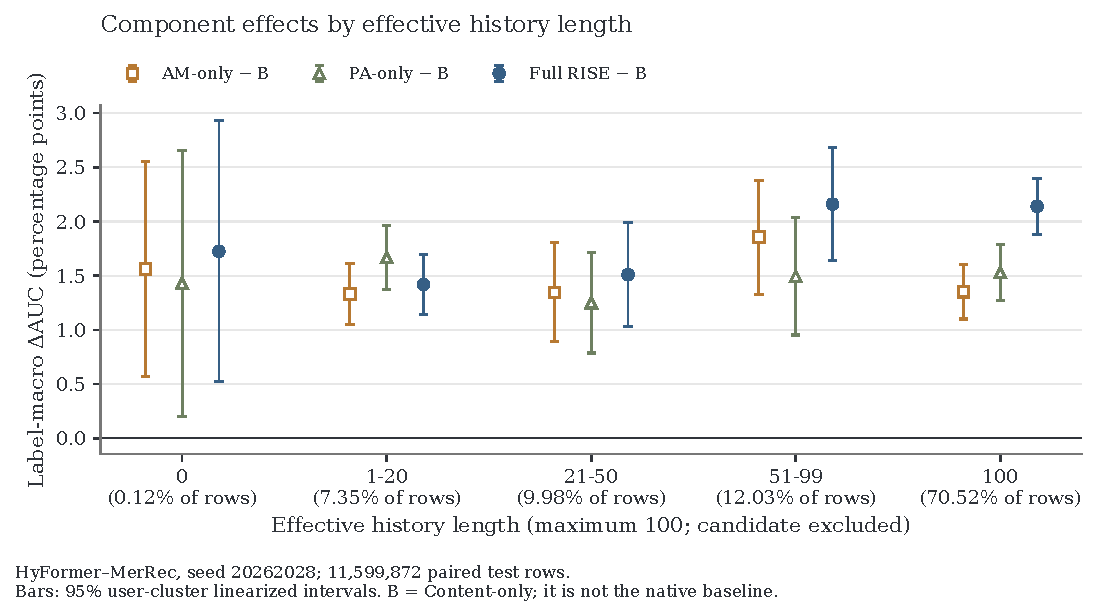
\includegraphics[width=0.97\textwidth]{figures/component_effect_by_history.pdf}
\caption{Verified component effects by effective history length. In the figure,
B denotes Content-only. Points compare independently trained component
configurations; bars are nominal user-cluster intervals, not training-seed
intervals. The vertical axis uses AUC percentage points, whereas the tables
report absolute AUC differences.}
\label{fig:rise_history_conditions}
\end{figure*}

\begin{figure*}[t]
\centering
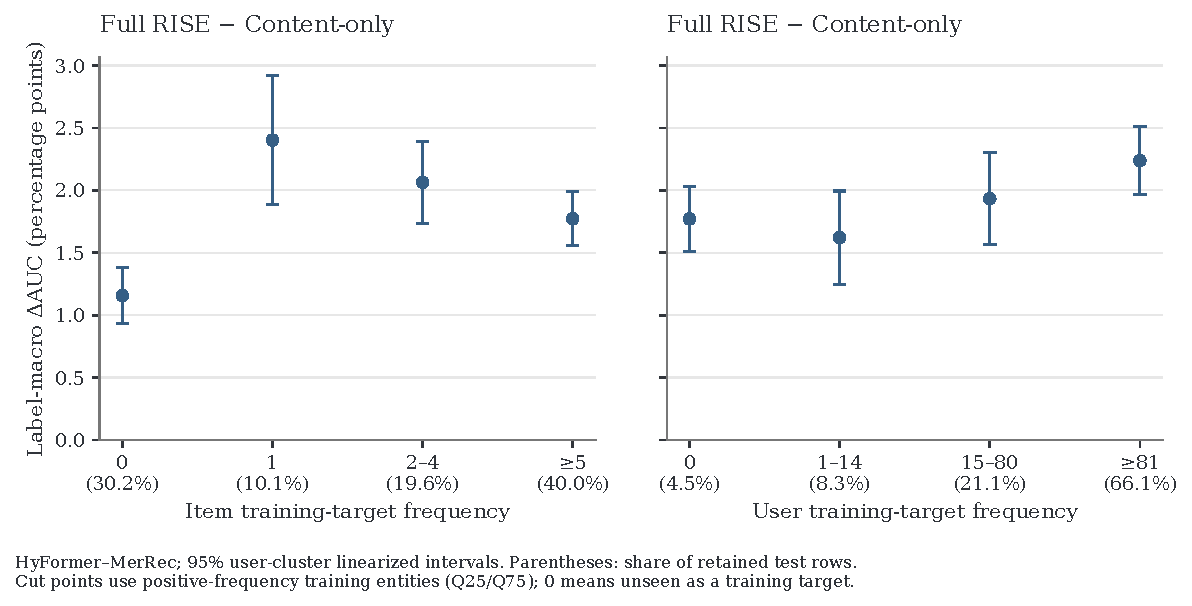
\includegraphics[width=0.97\textwidth]{figures/component_effect_by_frequency.pdf}
\caption{Full RISE minus Content-only by item and user training-target
frequency. Cut points use the positive-frequency entity distribution; parentheses
show retained sample shares. Marginal frequency comparisons do not separate
frequency from history length or other correlated properties.}
\label{fig:rise_frequency_conditions}
\end{figure*}
